\documentclass[10.5pt]{article}
\usepackage[top=4cm, bottom=4cm, left=4cm, right=4cm]{geometry}
\usepackage[utf8]{inputenc}
\usepackage[english]{babel}
\usepackage{amsmath}
\usepackage{graphicx}
\usepackage[T1]{fontenc}
\usepackage[natbibapa]{apacite}  % Keep apacite for bibliography style
\usepackage{hyperref}
\setcitestyle{notesep={:}}
\usepackage{booktabs, caption, longtable}
\usepackage{tabularx}
\usepackage{adjustbox}
\usepackage{pdfpages}
\usepackage{lmodern}  % Use Latin Modern Sans as the font
\usepackage{subcaption}
\usepackage{tabularx}
\usepackage{adjustbox}
\usepackage{fancyhdr}

\renewcommand{\familydefault}{\sfdefault}  % Set default font to sans-serif

\usepackage{tikz}
\usetikzlibrary{calc}
\newcommand\HRule{\rule{\textwidth}{1pt}}

% line spacing
\linespread{1.5}

% Use natbib for citation handling
\usepackage{natbib}
%\bibliographystyle{apalike}
\bibliographystyle{apacite} % Choose your desired bibliography style here

\begin{document}

\renewcommand{\refname}{Bibliography}

\begin{titlepage}

\begin{center}

% Upper part of the page
\textsc{\LARGE Universiteit Utrecht}\\[2.5cm]

\textsc{\Large Methodology \& Statistics for the Behavioural, Biomedical and Social Sciences}\\[1cm]
\textsc{\large Bayesian Statistics}\\[1cm]
% Title
\HRule \\[0.4cm]
{ \LARGE \bfseries Bayesian Data Integration using Metropolis Sampler with a Normal Approximation of the Posterior Distribution}\\[0.4cm]

\HRule \\[4cm]
\begin{minipage}{0.45\textwidth}
\begin{flushleft} \large
\emph{Author:}\\
Florian \textsc{Metwaly} \\
Student-Nr.: 0778265
\end{flushleft}
\end{minipage}
\begin{minipage}{0.45\textwidth}
\begin{flushright} \large
\emph{Lecturers:} \\
Noémi \textsc{Schuurman} \\
Herbert \textsc{Hoijtink} 
\end{flushright}
\end{minipage}

\vfill

% Bottom of the page
{\large July 19, 2024} \\

\end{center}

\end{titlepage}


\tableofcontents
\newpage

\section{Introduction}
In all fields of statistics, probability survey data is the gold standard of estimation and causal inference. Probability survey data describes a dataset, that is acquired by a sampling procedure in which the probabilities of drawing a person are known. Non probability samples (NPS) describe samples in which this probability is not known for every member of the population. While probability samples (PS) count as the gold standard, there are many good reasons not to use probability survey data. Non probability surveys are often cheaper, and it is possible to gain larger samples with less expense. In this report, I will explore a Bayesian data integration approach, which uses NPS data as prior information to enrich PS data to gain a better estimate of the population estimates. The approach is shown with the example of a logistic regression with two predictors, and the samples are drawn from a simulated population. The procedure follows the process as described in \cite{salvatore2024bayesian}. \\
The following report consists of four parts. First, I'll provide arguments why a Bayesian approach to data integration could be superior over a frequentist approach, next I will explain the simulation process, then I will explain how the model was estimated and lastly I will do a hypothesis test to test the estimated parameters against the population parameters. 

\section{Bayesian Data Integration}
Data integration is a big and recent topic in statistics. Frequentist procedures are most often based on weighting, which requires a range of covariates to be able to accurately describe the population and estimate their propensity scores. These covariates need to be present in both datasets that are supposed to be combined. This Bayesian approach does not need these covariates, as the data integration process is solely based on variables that are part of the analysis. This makes this approach more flexible and less prone to errors that occur when the covariates to create weights are selected, by not selecting the right variables to accurately describe the population.

\section{Simulation}
To be able to evaluate the estimation, a population is first simulated, then a PS sample is drawn with simple random sampling (n = 500) without replacement (srswr) and finally a NPS sample is drawn (n = 2000), with first giving a higher weight (1.3) to population members with the variable X1 = 1, to create a bias. This is a realistic scenario, for example, if a NPS is distributed through the internet. Having internet then is a prerequisite of being able to be drawn into the NPS, therefore not everyone has the same probability of being in the sample. \\
The simulated population has a size of 1 million and the population parameters \(\beta = (\beta_0, \beta_1, \beta_2)\) are defined as follows:
\begin{equation}
    \beta \in (0.5, 0.8, 0.3)
\end{equation}
All parameters and the population size were chosen somewhat arbitrarily. The sample sizes for the PS and NPS were picked to represent a realistic scenario, with a smaller PS and a larger but biased NPS.

\section{Estimation}
For Bayesian estimation, normally a sampler is needed, because of the complexity of the posterior distribution. The high complexity prevents an analytical solution.\\
Typical samplers are Gibbs, MCMC or Metropolis Hastings. Here, a Metropolis Sampler was used. A metropolis sampler is a special case of a Metropolis Hastings sampler, I will explain that later. \
Metropolis Hastings (MH) sampler first use a Markov-Chain-Monte-Carlo (MCMC) procedure to sample values from a proposal distribution, then apply a decision making rule if that proposed value is accepted or rejected. All accepted values form the posterior distribution \cite{chib1995understanding}. \\
Following, an MH is introduced which forms a posterior distribution out of the likelihood of the binary outcome variable and the so-called power prior. The power prior is a informative prior, using historical information to form a posterior distribution \citep{ibrahim2015power}. As proposed by \cite{salvatore2024bayesian}, here the NPS data is used as historical information in the power prior to integrate the data of the NPS into the PS. \\
The likelihood given the binary outcome variable is defined as
\begin{equation}
    L(Y|\beta_p) = p_i^{yi}(1-p_i^{yi})
\end{equation}
As the outcome is binary, a link function used to fit a generalized linear model \citep{mccullagh2019generalized}. The link function defines
\begin{equation}
    p_i = \frac{1}{1+e^{\beta_0 + x1\beta_1 + x2\beta_2}}
\end{equation}
Following the example of \cite{salvatore2024bayesian} the power prior 
\begin{equation}
    \pi(\beta, \alpha | Y_{nps}) \propto (L(Y_{nps}|\beta_p))^{\alpha}\pi_0(\beta_p|Y, \nu_0, \mu_0, \sigma_0)
\end{equation}
with the baseline prior \(\pi_0\) being a t-prior distribution which is simplified to
\begin{equation}
    \pi_0(\beta_p|Y, \nu_0, \mu_0, \sigma_0) = (1+\frac{1}{\nu_0}(\frac{\beta_p - \mu_0}{\sigma_0})^2)^{-\frac{\nu_0+1}{2}}
\end{equation}
is used. \\
The \(\alpha\) parameter describes the weight that is given to the historical information. Here, a Hotellings \(T^2\) is computed to compare the maximum likelihood estimates of the PS and the NPS. The p-value from that test describes the \(\alpha\) parameter. A p-value closer to 1 describes strong similarity of the estimates, therefore borrowing more data from the NPS, a p-value closer to 0 describes a large difference between the estimates and therefore leads to borrowing less data from the NPS \citep{salvatore2024bayesian}. \\
Using Bayes theorem, the posterior distribution therefore is proportional to
\begin{equation}
    \pi(\beta_p, \nu_0, \mu_0, \sigma_0|Y) \propto L(Y_{ps}|\beta_p)(L(Y_{nps}|\beta_p))^{\alpha}\pi_0(\beta_p|Y, \nu_0, \mu_0, \sigma_0)
\end{equation}
. \\
For the proposal distribution, a normal approximation of the posterior distribution was chosen. The normal approximation is defined as follows:
\begin{equation}
    q(\beta^*) = \mathcal{N}(\hat{\beta}_p, \hat{\sigma}_{\beta}^2) 
\end{equation}
\( \hat{\beta}_p \) is the estimated mode of the conditional posterior distribution. This mode was approximated numerically by using the optimise function in R. The variance \(\hat{\sigma}_{\beta}^2\) is minus the inverse of the fisher information \( \mathcal{I}(\hat{\beta}_p) \), estimated by first taking the logarithm of the conditional posterior,
\begin{equation}
    \begin{split}
        &\sum \left[ y_{i_{ps}} \ln \left( \frac{1}{1+\mathrm{e}^{-(\beta_{0_{ps}} + \beta_{1_{ps}} x_{1i_{ps}} + \beta_{2_{ps}} x_{2i_{ps}})}} \right) 
        + (1-y_{i_{ps}}) \ln \left( 1 - \frac{1}{1+\mathrm{e}^{-(\beta_{0_{ps}} + \beta_{1_{ps}} x_{1i_{ps}} + \beta_{2_{ps}} x_{2i_{ps}})}} \right) \right] \\
        &+\alpha \sum \left[ y_{i_{nps}} \ln \left( \frac{1}{1+\mathrm{e}^{-(\beta_{0_{nps}} + \beta_{1_{nps}} x_{1i_{nps}} + \beta_{2_{nps}} x_{2i_{nps}})}} \right) 
        + (1-y_{i_{nps}}) \ln \left( 1 - \frac{1}{1+\mathrm{e}^{-(\beta_{0_{nps}} + \beta_{1_{nps}} x_{1i_{nps}} + \beta_{2_{nps}} x_{2i_{nps}})}} \right) \right] \\
        &+ \frac{-(\nu_0+1)}{2} \ln \left( 1 + \frac{(\beta_p - \mu_0)^2}{\nu_0 \sigma_0^2} \right)
    \end{split}
\end{equation}
then taking the first derivative in respect to \( \hat{\beta}_p \)
\begin{equation}
    \begin{split}
        &\sum \left[ y_{i_{ps}} \frac{1}{1+\mathrm{e}^{\beta_{0_{ps}} + \beta_{1_{ps}} x_{1i_{ps}} + \beta_{2_{ps}} x_{2i_{ps}}}} 
        + (y_{i_{ps}} - 1) \frac{\mathrm{e}^{\beta_{0_{ps}} + \beta_{1_{ps}} x_{1i_{ps}} + \beta_{2_{ps}} x_{2i_{ps}}}}{1+\mathrm{e}^{\beta_{0_{ps}} + \beta_{1_{ps}} x_{1i_{ps}} + \beta_{2_{ps}} x_{2i_{ps}}}} \right] \\
        &+ \alpha \sum \left[ y_{i_{nps}} \frac{1}{1+\mathrm{e}^{\beta_{0_{nps}} + \beta_{1_{nps}} x_{1i_{nps}} + \beta_{2_{nps}} x_{2i_{nps}}}} 
        + (y_{i_{nps}} - 1) \frac{\mathrm{e}^{\beta_{0_{nps}} + \beta_{1_{nps}} x_{1i_{nps}} + \beta_{2_{nps}} x_{2i_{nps}}}}{1+\mathrm{e}^{\beta_{0_{nps}} + \beta_{1_{nps}} x_{1i_{nps}} + \beta_{2_{nps}} x_{2i_{nps}}}} \right] \\
        &+ \frac{(\nu_0 + 1) (\beta_p^2 - \mu_0)}{(\beta_p - \mu_0)^2 + \nu_0 \sigma_0^2}
    \end{split}
\end{equation}
\begin{equation}
    \begin{split}
        &\sum \left[ y_{i_{ps}} x_{\frac{1}{2}i_{ps}} \frac{1}{1+\mathrm{e}^{\beta_{0_{ps}} + \beta_{1_{ps}} x_{1i_{ps}} + \beta_{2_{ps}} x_{2i_{ps}}}} 
        + (y_{i_{ps}} - 1) x_{\frac{1}{2}i_{ps}} \frac{\mathrm{e}^{\beta_{0_{ps}} + \beta_{1_{ps}} x_{1i_{ps}} + \beta_{2_{ps}} x_{2i_{ps}}}}{1+\mathrm{e}^{\beta_{0_{ps}} + \beta_{1_{ps}} x_{1i_{ps}} + \beta_{2_{ps}} x_{2i_{ps}}}} \right] \\
        &+ \alpha \sum \left[ y_{i_{nps}} x_{\frac{1}{2}i_{nps}} \frac{1}{1+\mathrm{e}^{\beta_{0_{nps}} + \beta_{1_{nps}} x_{1i_{nps}} + \beta_{2_{nps}} x_{2i_{nps}}}} 
        + (y_{i_{nps}} - 1) x_{\frac{1}{2}i_{nps}} \frac{\mathrm{e}^{\beta_{0_{nps}} + \beta_{1_{nps}} x_{1i_{nps}} + \beta_{2_{nps}} x_{2i_{nps}}}}{1+\mathrm{e}^{\beta_{0_{nps}} + \beta_{1_{nps}} x_{1i_{nps}} + \beta_{2_{nps}} x_{2i_{nps}}}} \right] \\
        &+ \frac{(\nu_0 + 1) (\beta_p^2 - \mu_0)}{(\beta_p - \mu_0)^2 + \nu_0 \sigma_0^2}
    \end{split}
\end{equation}

and second derivative
\begin{equation}
    \begin{split}
        &\sum \left[ y_{i_{ps}} \frac{\mathrm{e}^{\beta_{0_{ps}} + \beta_{1_{ps}} x_{1i_{ps}} + \beta_{2_{ps}} x_{2i_{ps}}}}{(1+\mathrm{e}^{\beta_{0_{ps}} + \beta_{1_{ps}} x_{1i_{ps}} + \beta_{2_{ps}} x_{2i_{ps}}})^2} 
        + (y_{i_{ps}} - 1) \frac{\mathrm{e}^{\beta_{0_{ps}} + \beta_{1_{ps}} x_{1i_{ps}} + \beta_{2_{ps}} x_{2i_{ps}}}}{(1+\mathrm{e}^{\beta_{0_{ps}} + \beta_{1_{ps}} x_{1i_{ps}} + \beta_{2_{ps}} x_{2i_{ps}}})^2} \right] \\
        &+ \alpha \sum \left[ y_{i_{nps}} \frac{\mathrm{e}^{\beta_{0_{nps}} + \beta_{1_{nps}} x_{1i_{nps}} + \beta_{2_{nps}} x_{2i_{nps}}}}{(1+\mathrm{e}^{\beta_{0_{nps}} + \beta_{1_{nps}} x_{1i_{nps}} + \beta_{2_{nps}} x_{2i_{nps}}})^2} 
        + (y_{i_{nps}} - 1) \frac{\mathrm{e}^{\beta_{0_{nps}} + \beta_{1_{nps}} x_{1i_{nps}} + \beta_{2_{nps}} x_{2i_{nps}}}}{(1+\mathrm{e}^{\beta_{0_{nps}} + \beta_{1_{nps}} x_{1i_{nps}} + \beta_{2_{nps}} x_{2i_{nps}}})^2} \right] \\
        &+ \frac{(\nu_0 + 1)((\beta_p - \mu_0)^2 - \nu_0 \sigma_0^2)}{\left((\beta_p - \mu_0)^2 + \nu_0 \sigma_0^2\right)^2}
    \end{split}
\end{equation}
\begin{equation}
    \begin{split}
        &\sum \left[ y_{i_{ps}} x_{1/2i_{ps}} 
        \frac{\mathrm{e}^{\beta_{0_{ps}} + \beta_{1_{ps}} x_{1i_{ps}} + \beta_{2_{ps}} x_{2i_{ps}}}}{\left(1+\mathrm{e}^{\beta_{0_{ps}} + \beta_{1_{ps}} x_{1i_{ps}} + \beta_{2_{ps}} x_{2i_{ps}}}\right)^2} \right. \\
        &\left. + (y_{i_{ps}} - 1) x_{1/2i_{ps}} 
        \frac{\mathrm{e}^{\beta_{0_{ps}} + \beta_{1_{ps}} x_{1i_{ps}} + \beta_{2_{ps}} x_{2i_{ps}}}}{\left(1+\mathrm{e}^{\beta_{0_{ps}} + \beta_{1_{ps}} x_{1i_{ps}} + \beta_{2_{ps}} x_{2i_{ps}}}\right)^2} \right] \\
        &+ \alpha \sum \left[ y_{i_{nps}} x_{1/2i_{nps}} 
        \frac{\mathrm{e}^{\beta_{0_{nps}} + \beta_{1_{nps}} x_{1i_{nps}} + \beta_{2_{nps}} x_{2i_{nps}}}}{\left(1+\mathrm{e}^{\beta_{0_{nps}} + \beta_{1_{nps}} x_{1i_{nps}} + \beta_{2_{nps}} x_{2i_{nps}}}\right)^2} \right. \\
        &\left. + (y_{i_{nps}} - 1) x_{1/2i_{nps}} 
        \frac{\mathrm{e}^{\beta_{0_{nps}} + \beta_{1_{nps}} x_{1i_{nps}} + \beta_{2_{nps}} x_{2i_{nps}}}}{\left(1+\mathrm{e}^{\beta_{0_{nps}} + \beta_{1_{nps}} x_{1i_{nps}} + \beta_{2_{nps}} x_{2i_{nps}}}\right)^2} \right] \\
        &+\frac{(\nu_0+1)\left((\beta_p-\mu_0)^2-\nu_0\sigma_0^2\right)}{\left((\beta_p-\mu_0)^2+\nu_0\sigma_0^2\right)^2}
    \end{split}
\end{equation}

and finally by taking minus the inverse, resulting in
\[\hat{\sigma}_{\beta}^2 = -\frac{1}{\mathcal{I}(\hat{\beta}_p)} \]
. \\
Given that the proposal distribution is symmetric, the acceptance ratio can be simplified to
\begin{equation}
    r = \frac{\pi(\beta^{*})}{\pi(\beta_{t-1})}\frac{q(\beta^{*})}{q(\beta_t-1)} = \frac{\pi(\beta^{*})}{\pi(\beta_{t-1})}
\end{equation}
because 
\begin{equation}
    q(\beta^{*}) = q(\beta_{t-1})
\end{equation}
This special case is simply called a metropolis sampler. \\

\subsection{Results}
The sampler is run with 3 chains, with each chain sampling 10000 times. The baseline prior is defined as mildly informative as proposed by \cite{salvatore2024bayesian} with the parameters \(\mu_0 = 0, \sigma_0 = 2.5, \nu_0 = 3\). The first 3000 samples were removed as burn in period. Starting values \(\beta_p\) are \(beta_0 = 1, \beta_1 = 2, \beta_2 = 3\). Through all sampling processes, a seed is set to ensure reproducibility.
Finally, running the sampler and estimating the parameters \(beta_0, \beta_1\) and \(\beta_2\) leads to the results shown in Table 1.
\begin{table}[ht]
    \centering
    \caption{Estimates, 95\% Credible Intervals, and MSE for Logistic Regression Coefficients}
    \begin{tabular}{lccc}
        \toprule
        & Estimate & 95\% Credible Interval & MSE(\(\hat{\beta_p}\)) \\
        \midrule
        $\beta_0$ & 0.47 & [0.21; 0.73] & 0.0183 \\
        $\beta_1$ & 0.83 & [0.60; 1.07] & 0.0154 \\
        $\beta_2$ & 0.40 & [0.18; 0.62] & 0.0225 \\
        \bottomrule
    \end{tabular}
\end{table}
The trace plots in Figure 1 to 3 show that all three chains converged well. \\
\begin{figure}[htbp]
  \centering
  \begin{minipage}[b]{0.3\textwidth}
    \centering
    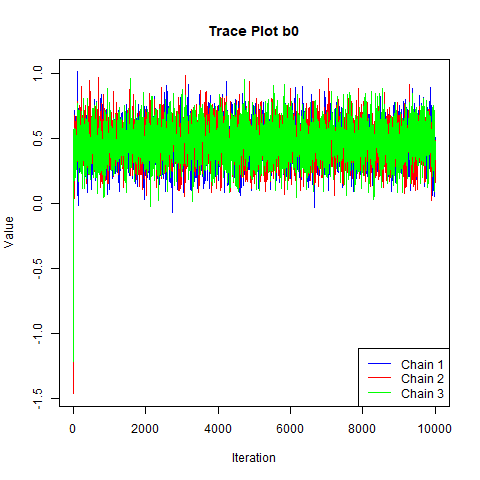
\includegraphics[width=\textwidth]{../results/trace_plot_b0.png}
    \caption{Traceplot \(\beta_0\)}
    \label{fig:traceplot1}
  \end{minipage}
  \hfill
  \begin{minipage}[b]{0.3\textwidth}
    \centering
    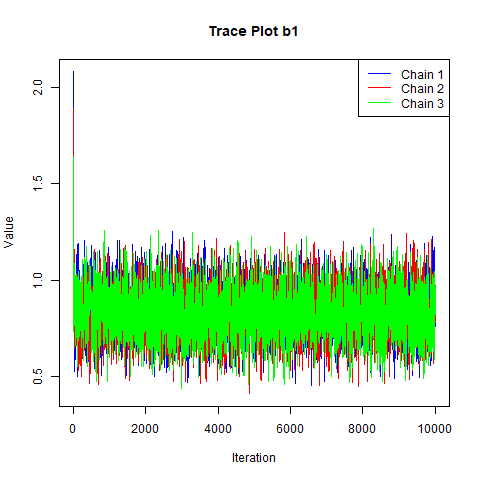
\includegraphics[width=\textwidth]{../results/trace_plot_b1.png}
    \caption{Traceplot \(\beta_1\)}
    \label{fig:traceplot2}
  \end{minipage}
  \hfill
  \begin{minipage}[b]{0.3\textwidth}
    \centering
    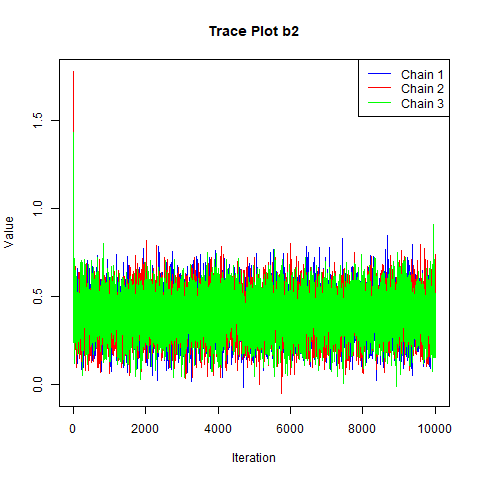
\includegraphics[width=\textwidth]{../results/trace_plot_b2.png}
    \caption{Traceplot \(\beta_2\)}
    \label{fig:traceplot3}
  \end{minipage}
\end{figure}
Further, the sampler has an acceptance rate of 0.9996, 0.9993 and 0.9998 for the three estimates respectively and each has an autocorrelation of 0.299.\\
Next to the estimates, Table 1 also shows the mean squared error (MSE), a measure quantifying the total survey error TSE as described in \cite{biemer2010total}. The MSE is calculated taking bias and variance of the sample into account.
\begin{equation}
    MSE(\hat{\beta_p}) = Bias^2(\hat{\beta_p}) + Var(\hat{\beta_p}) 
\end{equation}
A lower MSE can be interpreted as a better estimate. \\
The intercept \(\hat{\beta_0}\) is estimated to be 0.47 with a 95\% CI from 0.21 to 0.73. The MSE is 0.0183, showing that the estimate is very close to the population parameter \(\beta_0 = 0.5\). \(\hat{\beta_1}\) is estimated with 0.83 with a 95\% CI from 0.6 to 1.07 and an MSE of 0.0154, again confirming a good estimate close to the population parameter \(\beta_1 = 0.8\). Lastly, \(\hat{\beta_2}\) is estimated to be 0.4, with a 95\% CI of 0.18 to 0.62 and an MSE of 0.0225. The population parameter \(\beta_2 = 0.3\) was again well estimated. All three parameters show somewhat large credible intervals. Further analyses could investigate if a different baseline prior or a different estimation of the \(\alpha\) parameter of the power prior can lead to a closer estimation of the credible intervals. \\
In the following section a Bayesian hypothesis testing framework is used to compare the estimates to the population parameters.

\section{Bayesian Hypothesis Testing}
In the following section the $R$-package $bain$ \citep{gu2019bain} is used to perform a test of the estimated parameter against the population parameter. A Bayes Factor is computed to test the hypothesis \(\hat{\beta_p} = \beta_p\). The Bayes Factor is a quantification of the support for \(H_1\)  over the unconstrained hypothesis \(H_u\). It is computed by dividing the marginal likelihoods the hypotheses
\begin{equation}
    BF_{1u} = \frac{m_1}{m_u} = \frac{fit_1}{complexity_1}
\end{equation}
when the hypotheses are nested, the Bayes Factor can be computed solely through the fit and complexity of \(H_1\) \citep{hoijtink2011informative}. Table 2 shows the results of the Bayesian hypothesis tests.
\begin{table}[htbp]
    \centering
    \begin{adjustbox}{width=1.2\textwidth,center}
    \begin{tabularx}{\textwidth}{l *{7}{>{\centering\arraybackslash}X}}
        \toprule
        & Fit & Com & BF.u & BF.c & PMPa & PMPb & PMPc \\
        \midrule
        \textbf{\(H_1: \hat{\beta_0} = 0.5\)} & & & & & & & \\
        \(H_1\) & 2.947 & 0.061 & 48.657 & 48.657 & 1.000 & 0.980 & 0.980 \\
        \(H_u\) & & & & & 0.020 & & \\
        \(H_c\) & & & & & & 0.020 & \\
        \midrule
        \textbf{\(H_1: \hat{\beta_1} = 0.8\)} & & & & & & & \\
        \(H_1\) & 3.206 & 0.067 & 47.963 & 47.963 & 1.000 & 0.980 & 0.980 \\
        \(H_u\) & & & & & 0.020 & & \\
        \(H_c\) & & & & & & 0.020 & \\
        \midrule
        \textbf{\(H_1: \hat{\beta_2} = 0.3\)} & & & & & & & \\
        \(H_1\) & 2.417 & 0.070 & 34.333 & 34.333 & 1.000 & 0.972 & 0.972 \\
        \(H_u\) & & & & & 0.028 & & \\
        \(H_c\) & & & & & & 0.028 & \\
        \bottomrule
    \end{tabularx}
    \end{adjustbox}
    \caption{Bayesian Hypothesis Test Results}
    \label{tab:bayesian-results}
\end{table}

The first part show the hypothesis test for the hypothesis \(\hat{\beta_0} = 0.5\). The Bayes Factor is 48.66, saying that there is 48.66 times the amount of support in favour of the hypothesis against the unconstrained hypothesis. The posterior model probability is 0.98. The posterior model probabilities can be interpreted as Bayesian error probabilities, as counterparts to the frequentist Type I and Type II error rates. With a certainty of 98\% the hypothesis \(\hat{\beta_0} = 0.5\) can be accepted. The second part shows the BF and PMP for hypothesis \(\hat{\beta_1} = 0.8\). The Bayes Factor is 47.96 and the PMP again is 0.98. The same conclusion as with the previous hypothesis can be drawn. Lastly, \(\hat{\beta_2} = 0.3\) shows a smaller Bayes Factor of 34.33 and a PMP of 0.97. Although slightly less supported, there is still a large amount of evidence that in all three cases the hypothesis \(\hat{\beta_p} = \beta_p\) can be accepted.

\section{Reflection}
To show a Bayesian data integration approach, a bayesian logistic regression model estimating a binary outcome variable with two predictors was run on two integrated data sets, drawn from the same population, using a Metropolis sampler. Further, the viability of the estimates was tested using a Bayesian hypothesis testing framework. \\
The estimation and the hypothesis test do indicate that this approach to data integration is viable and gives good estimates to the population parameters. The slightly worse estimate for the \(\beta_2\) parameter probably results from the \(x_2\) variable being used to create the weight with which the biased NPS was sampled. Further research can compare differently strong biased non probability samples and different sample sizes, as well as different amounts of parameters.



\newpage


\bibliography{bibliography}

\newpage

\pagestyle{fancyplain}
\vspace*{\fill}
     \begin{center}
          \bf{\Huge{Appendices}}
     \end{center}
\vspace*{\fill}
\thispagestyle{fancy}

\makeatletter
\def\@makechapterhead#1{%
  \vspace*{30\p@}%
  {\noindent\LARGE\bf APPENDIX\ \thechapter \hspace*{0.5cm} \parindent \z@ \raggedright \normalfont
    \interlinepenalty\@M
    \LARGE \bfseries #1\par\nobreak
    \vskip 30\p@
  }}
  \makeatother
  
\appendix
\thispagestyle{empty}
\pagenumbering{gobble}


\end{document}